%
% Exemplo LaTeX de artigo UNISINOS
%
% Elaborado com base nas orientações dadas no documento
% ``GUIA PARA ELABORAÇÃO DE TRABALHOS ACADÊMICOS''
% disponível no site da biblioteca da Unisinos.
% http://www.unisinos.br/biblioteca
% 
% Os elementos textuais abaixo são apresentados na ordem em que devem
% aparecer no documento.  Repare que nem todos são obrigatórios - isso
% é devidamente indicado em cada caso.
%
% Comentários abaixo colocados entre aspas (`` '') foram
% extraídos diretamente do documento da biblioteca.
%
% Este documento é de domínio público.
%

%=======================================================================
% Declarações iniciais identificando a classe de documento e
% selecionando alguns pacotes adicionais.
%
% As opções disponíveis (separe-as com vírgulas, sem espaço) são:
% - twoside: Formata o documento para impressão frente-e-verso
%   (o default é somente-frente)
% - english,brazilian,french,german,etc.: idiomas usados no documento.
%   Deve ser colocado por último o idioma principal.
%=======================================================================
\documentclass[english,brazilian]{UNISINOSartigo} %twoside
\usepackage[utf8]{inputenc} % charset do texto (utf8, latin1, etc.)
\usepackage[T1]{fontenc} % encoding da fonte (afeta a sep. de sílabas)
\usepackage{graphicx} % comandos para gráficos e inclusão de figuras
\usepackage{bibentry} % para inserir refs. bib. no meio do texto
\usepackage{float}
\usepackage{array}
\usepackage{tabularx}
\usepackage{booktabs}
\usepackage{multirow}
\usepackage{newfloat}
\usepackage{setspace}
\usepackage{enumitem}
\usepackage{placeins}
%\usepackage{longtable}

\DeclareFloatingEnvironment[
fileext=loq,
listname={Lista de Quadros},
name=Quadro,
%placement=p,
%within=section,
%chapterlistsgaps=off
]{quadro}

\newcolumntype{L}{>{\centering\arraybackslash}m{6.2cm}}
\newcolumntype{G}{>{\centering\arraybackslash}m{5.5cm}}
\newcolumntype{A}{>{\centering\arraybackslash}m{2.4cm}}
\newcolumntype{B}{>{\centering\arraybackslash}m{7.5cm}}
%=======================================================================
% Escolha do sistema para geração de referências bibliográficas.
%
% O default é usar o estilo unisinos.bst.  Comente a definição abaixo
% e descomente a linha seguinte para usar o estilo do ABNTeX (é
% necessário ter esse pacote instalado).
%
% A vantagem do unisinos.bst é que ele permite o uso de um arquivo .bib
% seguindo as orientações tradicionais do BibTeX (veja essas orientações
% em http://ctan.tug.org/tex-archive/biblio/bibtex/contrib/doc/btxdoc.pdf).
% Entretanto, o estilo não suporta algumas citações mais exóticas como
% apud.  Para isso, use o ABNTeX, mas esteja ciente de que muitas de
% suas referências serão incompatíveis com os estilos tradicionais do
% BibTeX como plain, alpha, ieeetr, entre outros.
%=======================================================================
\usepackage[alf]{abntex2cite}

\autor{CLOSS FRAGA}{GUILHERME}
\titulo{O Impacto da Inteligência Artificial no Processo de Desenvolvimento de \textit{Software}:}
\subtitulo{Um estudo comparativo entre desenvolvedores com e sem o uso de ferramentas de IA}
\orientador[Prof.ª Dra.]{Francisco}{Rosemary}
%\coorientador[Prof.~Dr.]{Lamport}{Leslie}
\local{São Leopoldo}
\ano{2025}
\unidade{Unidade Acadêmica de Graduação}
\curso{Curso de Bacharelado em Ciência da Computação}
\natureza{%
Artigo apresentado como requisito parcial para obtenção do título de Bacharel em Ciência da Computação, pelo Curso de Ciência da Computação da Universidade do Vale do Rio dos Sinos (UNISINOS)}

%=======================================================================
% Início do documento.
%=======================================================================

\begin{document}
\capa
\folhaderosto

% Diferentemente do normal, os comandos a seguir devem vir aqui mesmo,
% e não antes do \begin{document} onde seria o lugar deles. 
\tituloArtigo{O Impacto da Inteligência Artificial no Processo de Desenvolvimento de \textit{Software}:}{Um estudo comparativo entre desenvolvedores com e sem o uso de ferramentas de IA}
\autorArtigo{Guilherme Closs Fraga\footnote{Graduando em Ciência da Computação pela Unisinos.  Email: guifraga8@edu.unisinos.br}}
\autorArtigo{Rosemary Francisco\footnote{Doutora em Administração. Email: rosemaryf@unisinos.br}}

%=======================================================================
% Resumo em Português.
%
% A recomendação é para 150 a 250 palavras.
%=======================================================================
\begin{abstract}
Lorem ipsum.

\palavraschave{lorem ipsum.}
\end{abstract}

\begin{otherlanguage}{english}
\singlespacing
\begin{abstract}
Lorem ipsum.
\end{abstract}
\palavraschave{lorem ipsum.}
\end{otherlanguage}

%=======================================================================
% Introdução
%=======================================================================
\section{Introdução}

A Inteligência Artificial (IA) tem se consolidado como uma das tecnologias mais transformadoras da atualidade, conquistando espaço em diferentes setores da sociedade e despertando interesse tanto no meio acadêmico quanto no mercado. Trata-se do uso de algoritmos e modelos computacionais capazes de executar tarefas que, até pouco tempo atrás, dependiam exclusivamente da capacidade cognitiva humana, como análise de dados, raciocínio lógico e tomada de decisão. Esse avanço tem proporcionado mudanças significativas, especialmente no que se refere à automação e otimização de processos, abrindo novas possibilidades de atuação profissional e acadêmica.

No campo do desenvolvimento de \textit{software}, a presença da IA tornou-se ainda mais evidente. Ferramentas baseadas em técnicas de aprendizado de máquina e processamento de linguagem natural têm auxiliado desenvolvedores em diferentes etapas do ciclo de vida do \textit{software}, desde a escrita de código até a detecção de falhas e otimização de desempenho. Um exemplo é o \textit{GitHub Copilot}, lançado em 2021 pela \textit{GitHub} em parceria com a \textit{OpenAI}, que utiliza modelos de IA Generativa (também chamadas de IA Gen) para sugerir trechos de código em tempo real \cite{github2021}. Outra ferramenta amplamente utilizada é o próprio \textit{ChatGPT}, lançado pela \textit{OpenAI} em 2022, capaz de responder dúvidas técnicas, gerar soluções de programação e até apoiar na documentação de sistemas \cite{wikipedia2024}.

Esses recursos, ao mesmo tempo em que oferecem praticidade e aumentam a produtividade, também levantam debates relevantes. Há questionamentos sobre até que ponto a utilização dessas ferramentas pode impactar o aprendizado e a prática de programação, visto que os desenvolvedores podem se tornar excessivamente dependentes delas, deixando de aprimorar suas próprias habilidades de raciocínio lógico e resolução de problemas. Além disso, discute-se sobre a qualidade e a confiabilidade das soluções geradas pela IA, que nem sempre são isentas de erros ou falhas conceituais, exigindo do profissional uma postura crítica em relação ao uso dessas tecnologias \cite{rivas2025}.

Por outro lado, pesquisas recentes indicam que a adoção de IA no desenvolvimento de \textit{software} pode representar ganhos significativos em termos de produtividade e redução do tempo necessário para a entrega de soluções. Um estudo piloto com profissionais de \textit{software} demonstrou percepções majoritariamente positivas quanto ao impacto desses recursos na produtividade individual \cite{coutinho2024}. Essa realidade torna essencial a investigação de como essas ferramentas impactam o trabalho de desenvolvedores em contextos práticos. Assim, mais do que um recurso de conveniência, a IA se apresenta como um instrumento que pode redefinir processos e metodologias de engenharia de \textit{software}.

Neste contexto, este trabalho busca analisar comparativamente o desempenho de desenvolvedores em um desafio técnico, divididos em dois grupos: um com acesso a ferramentas de Inteligência Artificial e outro sem acesso a esses recursos. O objetivo é avaliar de que forma a utilização da IA influencia fatores como eficiência, qualidade do código e tempo de resolução do problema. Com isso, pretende-se fornecer uma visão crítica e fundamentada sobre as vantagens, limitações e implicações do uso dessas tecnologias no processo de desenvolvimento de \textit{software}.

A proposta deste estudo, portanto, está inserida no campo de Desenvolvimento de \textit{Software} propriamente, com enfoque no impacto das novas tecnologias sobre a prática profissional. Ao final, espera-se que os resultados obtidos contribuam para a compreensão dos reais benefícios e desafios da adoção da IA no desenvolvimento de \textit{software}, oferecendo resultados para pesquisadores, profissionais e instituições interessadas em compreender e orientar o uso dessas ferramentas emergentes.

\subsection{Proposta de Solução}

Atualmente, observa-se que o impacto da Inteligência Artificial no desenvolvimento de \textit{software} ainda é um tema em debate, sendo comum que as análises existentes se restrinjam a relatos de uso ou percepções subjetivas por parte dos desenvolvedores. Em muitos casos, a avaliação da influência da IA sobre fatores como produtividade, qualidade do código e tempo de execução de tarefas ocorre de forma fragmentada, sem um método padronizado que permita mensurar de maneira objetiva os efeitos reais de tais ferramentas.

Dentro desse cenário, este estudo propõe a elaboração de um desafio técnico, disponibilizado por meio de uma plataforma \textit{web} desenvolvida especificamente para este fim. Essa plataforma funcionará como um ambiente de avaliação controlado, no qual os participantes serão previamente organizados em dois grupos: um grupo com autorização para utilizar ferramentas de IA durante a resolução do desafio e outro grupo que deverá realizar a atividade sem recorrer a tais recursos.

A proposta busca, assim, criar condições equivalentes para ambos os grupos, garantindo que todos recebam o mesmo enunciado do desafio, apresentado diretamente na plataforma. Para cada participante será disponibilizado um link único, correspondente ao grupo ao qual pertence. A partir desse acesso, o desenvolvedor poderá visualizar as instruções, iniciar a tarefa e, ao concluir, submeter os arquivos com sua solução.

A plataforma também atuará como mecanismo de registro, armazenando automaticamente o tempo total gasto por cada participante, desde o momento em que deu início ao desafio até a finalização da entrega. Dessa forma, além da coleta da solução proposta, será possível analisar métricas objetivas como tempo de conclusão, qualidade do código entregue e eventuais diferenças de abordagem entre os grupos.

Em resumo, este trabalho busca responder à seguinte questão de pesquisa: de que maneira o uso de ferramentas de Inteligência Artificial Generativas impacta o desempenho de desenvolvedores de \textit{software} em atividades práticas de programação? Por meio da comparação entre os dois grupos, espera-se obter evidências consistentes que auxiliem na compreensão do papel da IA como aliada no processo de desenvolvimento de \textit{software}.

\subsection{Objetivos}

\subsubsection{Objetivo Geral}

O objetivo geral deste trabalho é analisar o impacto da utilização de ferramentas de IA Generativas no processo de desenvolvimento de \textit{software}, por meio da aplicação de um desafio técnico comparativo entre dois grupos de desenvolvedores, sendo um autorizado a utilizar recursos de IA e outro restrito ao desenvolvimento sem tais ferramentas. Sendo assim, será possível identificar diferenças em aspectos como produtividade, tempo de execução e qualidade das soluções entregues.

\subsubsection{Objetivos Específicos}

Abaixo, destacam-se os objetivos específicos necessários para atingir a conclusão deste trabalho:
\begin{enumerate}[label=\alph*), leftmargin=1.2cm, itemsep=0.1em, topsep=0.1em]
    \item desenvolver uma plataforma \textit{web} simples para disponibilização do desafio técnico e coleta de dados de desempenho dos participantes;
    \item aplicar o desafio técnico a dois grupos de desenvolvedores, sendo um autorizado a utilizar ferramentas de IA e outro restrito ao uso dessas tecnologias;
    \item comparar os resultados obtidos pelos grupos em relação ao tempo de conclusão, qualidade do código entregue e abordagem adotada na resolução do problema;
    \item analisar as vantagens, limitações e possíveis implicações do uso de ferramentas de IA no processo de desenvolvimento de \textit{software}.
\end{enumerate}

\section{Fundamentação Teórica}

Com base na temática que o presente trabalho visa abordar, se faz necessário discorrer sobre dois tópicos fundamentais para a construção e consolidação do mesmo, sendo eles: Desenvolvimento de \textit{Software} e IA Generativa aplicada ao desenvolvimento de \textit{software}. Nas seções seguintes, os conceitos são explorados e detalhados a fim de estabelecer os fundamentos teóricos necessários para compor este trabalho.

\subsection{Desenvolvimento de \textit{Software}}

Um \textit{software} refere-se a todos os componentes não físicos de um computador, redes de computadores ou dispositivos móveis. Em linhas gerais, refere-se aos programas e aplicações, como o próprio sistema operacional, que fazem aquele aparelho (ou ferramenta) operar de acordo com o que o usuário necessita. Isto é, \textit{software} se trata de uma coleção de instruções, dados ou programas utilizados para operar computadores e executar determinadas tarefas \cite{coutinho2021}.

Em outras palavras, pode-se dizer que é um termo genérico que se refere à aplicações, \textit{scripts} e programas executáveis em um determinado dispositivo. Assim, o diferencia de \textit{hardware}, que descreve os aspectos físicos de um aparelho. Sendo assim, podemos estabelecer o \textit{software} como um componente variável de um computador, enquanto o \textit{hardware} é constante \cite{sakurai2018}

De acordo com \citeonline{maynard2015}, temos basicamente dois tipos de \textit{software}, sendo eles: \textit{software} de aplicativo e \textit{software} de sistema. Um aplicativo seria aquele que atende uma necessidade específica ou executa determinadas tarefas. E, segundo \citeonline{schwab2019}, \textit{software} de sistema seria a parte essencial para que o \textit{hardware} de um computador opere, servindo como a plataforma para a execução de aplicativos. Ademais, podemos mencionar outros tipos de \textit{software}, como os de programação, que são ferramentas necessárias para desenvolvedores, \textit{middlewares}, responsáveis por atuarem entre o \textit{software} do sistema e aplicativos e até mesmo \textit{drivers}, que são responsáveis por operarem dispositivos e periféricos de computadores.

Por fim, a sincronia entre diferentes tipos de \textit{software} e \textit{hardware}, é peça fundamental para o funcionamento eficiente de sistemas computacionais. Enquanto um aplicativo permite que seus usuários realizem determinadas tarefas, um sistema assegura que o \textit{hardware} opere corretamente, dando suporte para diferentes aplicações. Com a constante crescente de complexidade em sistemas modernos, a presença de um \textit{middleware} eficaz se torna indispensável para assegurar que diferentes \textit{softwares} funcionem em harmonia. Da mesma forma que, \textit{drivers} são indispensáveis para comunicação entre o sistema e periféricos, o que amplia as funcionalidades de um computador, resultando na melhoria da experiência do usuário.

Sendo assim, os componentes técnicos de um computador são controlados por \textit{softwares}. Isto igualmente o difere do \textit{hardware} de um computador, rede ou dispositivo móvel, visto que ele não é fisicamente tangível. \citeonline{candido2022} diz que o sistema operacional nada mais é do que o \textit{software} fundamental de um computador ou dispositivo móvel. No que diz respeito aos termos de interface para o usuário, os três sistemas operacionais mais conhecidos, sendo eles \textit{Windows}, \textit{macOS} e \textit{Linux}, diferem. Outros programas e aplicações podem servir como complemento para as funções básicas de um sistema operacional. Eles podem ser instalados por meio de um \textit{driver} ou após \textit{download} e instalação. Estes programas incluem, por exemplo, o próprio \textit{MediaPlayer} ou \textit{Microsoft Office} da \textit{Microsoft} \cite{neto2019}.

Além dos sistemas operacionais, existe uma ampla gama de \textit{softwares} utilitários voltados para funções específicas que visam aprimorar tanto o desempenho quanto a segurança do computador. Entre eles, destacam-se os programas antivírus, as ferramentas de \textit{backup} e os aplicativos de manutenção de disco, que atuam na proteção das informações e na preservação da eficiência do sistema. Somado a isso, o avanço tecnológico possibilitou o surgimento dos \textit{softwares} de virtualização, que permitem a execução de diferentes sistemas operacionais em uma única máquina física, ampliando a flexibilidade e otimizando a utilização dos recursos de \textit{hardware}.

Em diversos dispositivos, o \textit{software} está diretamente integrado ao hardware, como ocorre em painéis eletrônicos de automóveis ou em máquinas de lavar. Exemplos comuns são os sistemas de navegação e os leitores de\textit{ Blu-Ray}, que funcionam sob controle de \textit{software}, mas não permitem substituição por alternativas diferentes. Segundo \citeonline{coutinho2021}, essas combinações fixas recebem a denominação de “embutidos”. Já na década de 1950, \textit{software} e \textit{hardware} eram concebidos como uma única unidade, em que o \textit{software} era tratado apenas como parte do \textit{hardware}, conhecido então como código de programa. Foi o estatístico John W. Tukey quem utilizou pela primeira vez o termo \textit{“software”} em 1958 \cite{maynard2015}. Conforme apontam \citeonline{sakurai2018}, somente cerca de vinte anos depois o governo dos Estados Unidos determinou que a IBM passasse a contabilizar seus componentes de \textit{hardware} e \textit{software} separadamente, decisão que abriu espaço para o fortalecimento de empresas especializadas no desenvolvimento de \textit{software}.

O avanço tecnológico tornou possível a dissociação entre \textit{software} e \textit{hardware}, proporcionando maior flexibilidade e impulsionando a inovação no desenvolvimento de sistemas computacionais. Essa separação permitiu que os programas fossem atualizados sem a necessidade de alterações no \textit{hardware}, acelerando os ciclos de inovação. A especialização na produção de \textit{software} também deu origem a uma indústria sólida, formada por empresas voltadas à criação de soluções personalizadas para diferentes setores e demandas. Esse movimento não só ampliou as formas de utilização dos dispositivos, como também favoreceu o surgimento de novos modelos de negócio baseados em \textit{software}, os quais desempenham papel central na atual economia digital.

\citeonline{schwab2019} destaca que o trabalho do programador consiste, de forma essencial, em traduzir requisitos e algoritmos para uma linguagem de programação que o computador consiga interpretar e executar. A partir desse processo, é possível desenvolver diferentes tipos de \textit{software}, como aplicativos, jogos e sistemas de controle para robôs. Um exemplo histórico ligado à ideia de programação foi a invenção de um \textit{tear} “programável” pelo francês Joseph-Marie Jacquard, que representou um marco na Revolução Industrial. O equipamento não possuía processador, sendo controlado por meio de cartões perfurados. Conforme explica \citeonline{maynard2015}, esses cartões não utilizavam valores binários como 0 e 1, mas funcionavam através da presença ou ausência de perfurações: um furo indicava uma ação de movimento, enquanto a ausência significava outra. A criação de Jacquard é considerada uma das precursoras da automação moderna.

\citeonline{maynard2015} aponta que, em 1843, Augusta Ada King-Noel, mais conhecida como Ada Lovelace, desempenhou um papel marcante ao colaborar com Charles Babbage no projeto do \textit{Analytical Engine}, uma calculadora mecânica de uso geral que acabou não sendo concluída. Durante esse processo, Ada elaborou diversas anotações e descreveu um método para calcular os números de Bernoulli por meio da máquina, o que, segundo \citeonline{coutinho2021}, é considerado o primeiro programa de computador da história. Posteriormente, em 1941, Konrad Ernst Otto Zuse desenvolveu o Z3, reconhecido como o primeiro sistema de computação totalmente automatizado e programável do mundo.

O Z3 foi construído a partir dos conceitos idealizados por Babbage e tinha como diferencial a capacidade de realizar operações, como a adição, em menos de um quarto de segundo. O propósito central de sua criação estava ligado à busca por maior eficiência nos cálculos. Nos primeiros anos, os \textit{softwares} eram desenvolvidos para máquinas específicas e eram comercializados em conjunto com o \textit{hardware}. Já na década de 1980, passaram a ser distribuídos em mídias físicas, como disquetes, e mais tarde em CDs e DVDs. Atualmente, grande parte dos \textit{softwares} é obtida por meio da \textit{Internet}, seja diretamente nos sites dos fabricantes ou através de plataformas de distribuição de aplicativos.

Os modelos de ciclo de vida de \textit{software} descrevem as etapas que um sistema percorre desde sua concepção até sua desativação, organizando a sequência de atividades necessárias para o desenvolvimento. O objetivo central desses modelos é garantir qualidade, reduzir custos e otimizar o tempo de entrega. Entre as fases mais comuns estão:

\begin{itemize}[leftmargin=1cm, itemsep=0.1em, topsep=0.1em]
    \item Análise de Requisitos: onde são levantadas e documentadas as necessidades do sistema;
    \item Design: define a arquitetura, fluxos de trabalho e tecnologias a serem utilizadas;
    \item Implementação: fase em que o código é desenvolvido com base no planejamento estabelecido;
    \item Testes: que envolvem diferentes tipos de verificação para assegurar a confiabilidade do \textit{software};
    \item Manutenção: responsável por corrigir falhas e implementar melhorias após a entrega do sistema. 
\end{itemize}

De acordo com \citeonline{candido2022}, observa-se nos últimos anos uma tendência de desprofissionalização no aprendizado de programação, já que muitas pessoas têm adquirido essas habilidades de forma autodidata, recorrendo a tutoriais \textit{online} em vez de cursos formais. Além disso, o \textit{networking} global, aliado às diversas plataformas digitais, tem favorecido a formação de grandes comunidades que reúnem tanto entusiastas quanto programadores experientes, tornando cada vez menos nítida a distinção entre esses grupos.

Ao mesmo tempo, percebe-se um avanço significativo nos padrões e na qualidade do desenvolvimento de \textit{software}. Os sistemas estão cada vez mais sofisticados e complexos, o que aumenta a demanda por soluções digitais. Esse contexto reflete uma sociedade em constante transformação, onde as necessidades mudam rapidamente, gerando uma procura crescente por Desenvolvedores \textit{Full Stack} (um profissional de tecnologia que possui a capacidade de trabalhar em todas as camadas de um projeto de \textit{software}) em detrimento de profissionais especializados apenas em uma área.

A complexidade crescente dos sistemas requer profissionais capazes de atuar em todas as camadas do desenvolvimento, abrangendo desde o \textit{Frontend} (interface do usuário) até o \textit{Backend} (servidor, banco de dados e lógica de negócios de uma aplicação). Nesse cenário, os Desenvolvedores \textit{Full Stack} ganham destaque por sua flexibilidade e capacidade de adaptação às mudanças do mercado e às demandas dos usuários. Sua habilidade em compreender e integrar diferentes componentes de um sistema favorece um desenvolvimento mais unificado e eficiente, além de melhorar a comunicação e colaboração dentro das equipes. Assim, em um ambiente em que a agilidade e a adaptabilidade são fatores essenciais, esses profissionais se consolidam como recursos estratégicos para empresas que buscam manter a competitividade.

O desenvolvimento de \textit{software} pode ser entendido como um conjunto de atividades voltadas ao projeto, criação, implementação e manutenção de programas que orientam o funcionamento de computadores, sendo independente do \textit{hardware} e responsável por torná-los programáveis \cite{schwab2019}. Segundo \citeonline{maynard2015}, esses programas podem ser classificados em três categorias principais:

\begin{itemize}[leftmargin=1cm, itemsep=0.1em, topsep=0.1em]
    \item \textit{Softwares} de sistema: englobam sistemas operacionais, utilitários e ferramentas de gerenciamento;
    \item \textit{Softwares} de programação: oferecem recursos como compiladores e depuradores para os desenvolvedores;
    \item \textit{Softwares} aplicativos: voltados ao usuário final, como ferramentas de produtividade, aplicativos de segurança e plataformas digitais, incluindo serviços online e aplicativos móveis. 
\end{itemize}

Outro tipo de \textit{software} é aquele voltado para sistemas embarcados, usados no controle de máquinas e dispositivos que nem sempre são reconhecidos como computadores, como redes telefônicas, veículos automotores e robôs industriais. Esses equipamentos, juntamente com seus \textit{softwares}, podem ser conectados dentro do ecossistema da Internet das Coisas (\textit{IoT}). Nesse contexto, programadores, engenheiros e desenvolvedores de \textit{software} exercem funções essenciais no desenvolvimento desses sistemas, com responsabilidades que frequentemente se sobrepõem e cuja dinâmica colaborativa pode variar dependendo do departamento ou da comunidade em que atuam.

As soluções de engenharia de \textit{software} baseiam-se em métodos científicos e precisam ser eficazes na prática, de forma semelhante a estruturas como pontes ou elevadores. À medida que os produtos se tornam mais inteligentes, incorporando microprocessadores, sensores e \textit{software}, a responsabilidade dos engenheiros de \textit{software} aumenta. Atualmente, a competitividade de um produto no mercado não depende apenas do \textit{software} que ele utiliza, mas da integração eficiente entre todos os seus componentes.

Conforme aponta \citeonline{candido2022}, o desenvolvimento de \textit{software} deve ser integrado ao desenvolvimento de produtos mecânicos e elétricos, o que faz com que o papel dos desenvolvedores de \textit{software} seja menos delimitado em comparação ao dos engenheiros. Esses profissionais podem focar em áreas específicas do projeto, como a codificação, enquanto o ciclo de vida do \textit{software} envolve a transformação de requisitos em funcionalidades, o trabalho em equipes multifuncionais, a gestão de processos e equipes, além de atividades de teste e manutenção.

De acordo com \citeonline{schwab2019}, a atuação dos desenvolvedores de \textit{software} vai além das equipes de programação, envolvendo também cientistas e fabricantes de dispositivos e \textit{hardware}, que contribuem para a criação de códigos, mesmo não sendo os principais responsáveis pelo desenvolvimento. Essa participação não se limita às indústrias tradicionais de tecnologia da informação, abrangendo também empresas que não se dedicam exclusivamente à produção de \textit{software} ou semicondutores.

A ampliação do papel dos desenvolvedores de \textit{software} evidencia a crescente integração da tecnologia da informação com diversas áreas, como ciência, medicina, engenharia e artes. Atualmente, o desenvolvimento de \textit{software} é fundamental para múltiplos setores, desde a indústria automotiva até o entretenimento, impulsionando a inovação e a transformação digital. Na indústria automotiva, esses profissionais são essenciais para o desenvolvimento de sistemas de condução autônoma e tecnologias avançadas de segurança. Já no cinema, os efeitos visuais e a animação digital dependem fortemente do \textit{software} para criar mundos e personagens realistas. Dessa forma, os desenvolvedores de \textit{software} exercem um papel cada vez mais diversificado e influente, moldando o futuro em diferentes áreas do conhecimento e da atividade humana.

\subsubsection{Modelos de Desenvolvimento de \textit{Software}}

O desenvolvimento de \textit{software} pode ser conduzido por diferentes abordagens, conhecidas como modelos de processo de \textit{software}. Esses modelos têm como objetivo estruturar e organizar as atividades necessárias para transformar requisitos em um produto final de qualidade. Entre os modelos mais conhecidos estão o Modelo Cascata, o Modelo em V, o Modelo Espiral e os Modelos Ágeis.

O Modelo Cascata (ou \textit{Waterfall}) foi um dos primeiros modelos formais de processo de software. Proposto por Winston Royce em 1970, consiste em uma sequência linear de fases: levantamento de requisitos, análise, projeto, implementação, testes, implantação e manutenção. Cada fase deve ser concluída antes do início da próxima, funcionando como uma “cascata” de atividades \cite{sommerville2011}. Entre suas vantagens podemos citar:

\begin{itemize}[leftmargin=1cm, itemsep=0.1em, topsep=0.1em]
    \item Estrutura simples e de fácil entendimento;
    \item Definição clara das fases e entregas;
    \item Útil em projetos com requisitos bem definidos e estáveis.
\end{itemize}

Por outro lado, há também desvantagens que valem ser destacadas deste modelo, sendo elas:

\begin{itemize}[leftmargin=1cm, itemsep=0.1em, topsep=0.1em]
    \item Pouca flexibilidade diante de mudanças nos requisitos;
    \item Risco de identificação tardia de falhas, geralmente apenas na fase de testes;
    \item Dificuldade em lidar com projetos complexos ou inovadores.
\end{itemize}

O Modelo em V é uma extensão do Modelo Cascata, mas com foco maior na validação e verificação em cada etapa do desenvolvimento. A representação em formato de “V” mostra que para cada fase de desenvolvimento existe uma fase correspondente de teste: requisitos são validados com testes de aceitação, projeto de sistema é validado com testes de integração, e assim sucessivamente \cite{pressman2016}. Entre suas principais vantagens, temos:

\begin{itemize}[leftmargin=1cm, itemsep=0.1em, topsep=0.1em]
    \item Ênfase na qualidade e no teste desde o início do processo;
    \item Adequado para sistemas críticos, como os da área médica ou aeroespacial.
\end{itemize}

Já como desvantagens, temos:

\begin{itemize}[leftmargin=1cm, itemsep=0.1em, topsep=0.1em]
    \item Semelhante ao Cascata, é rígido e pouco adaptável a mudanças;
    \item Elevado custo caso ocorra necessidade de alterações durante o desenvolvimento.
\end{itemize}

O Modelo Espiral, proposto por Barry Boehm em 1986, combina elementos do Modelo Cascata com técnicas de prototipação e gerenciamento de riscos. O desenvolvimento é representado como uma espiral, onde cada ciclo envolve: definição de objetivos, análise de riscos, desenvolvimento e validação, e planejamento da próxima iteração \cite{boehm1988}. Das vantagens deste modelo, ressaltam-se:

\begin{itemize}[leftmargin=1cm, itemsep=0.1em, topsep=0.1em]
    \item Forte ênfase na análise e mitigação de riscos;
    \item Flexibilidade para incorporar mudanças ao longo do processo;
    \item Permite versões incrementais do sistema.
\end{itemize}

E, como desvantagens temos:

\begin{itemize}[leftmargin=1cm, itemsep=0.1em, topsep=0.1em]
    \item Complexidade de gerenciamento maior do que em modelos lineares;
    \item Custo elevado, especialmente em projetos pequenos;
    \item Exige maior envolvimento de profissionais experientes em análise de riscos.
\end{itemize}

Os Modelos Ágeis surgiram como uma alternativa aos modelos tradicionais, sendo formalizados em 2001 com o Manifesto Ágil. Esses modelos priorizam colaboração com o cliente, entregas rápidas e contínuas, adaptação às mudanças e interações entre pessoas mais do que processos rígidos \cite{beck2001}.

Entre os métodos ágeis mais utilizados, principalmente nos dias atuais, estão o \textit{Scrum}, o \textit{Kanban} e o \textit{Extreme Programming} (conhecido também como \textit{XP}). Todos eles seguem o princípio de dividir o projeto em pequenos ciclos (iterações), resultando em entregas frequentes e incrementais do produto. Como as principais vantagens, podemos citar:

\begin{itemize}[leftmargin=1cm, itemsep=0.1em, topsep=0.1em]
    \item Alta flexibilidade para mudanças de requisitos;
    \item Entregas rápidas que geram valor contínuo ao cliente;
    \item Melhora na comunicação e na colaboração entre equipe e \textit{stakeholders}.
\end{itemize}

E, das suas principais desvantagens:

\begin{itemize}[leftmargin=1cm, itemsep=0.1em, topsep=0.1em]
    \item Pode gerar falta de documentação formal, dependendo da equipe;
    \item Requer alto envolvimento do cliente no processo;
    \item Menos indicado para projetos de missão crítica que demandam forte rastreabilidade.
\end{itemize}

Sendo assim, evidencia-se que cada modelo de desenvolvimento possui suas características, vantagens e limitações. A escolha do modelo mais adequado depende do contexto do projeto, da complexidade do sistema, do nível de risco, do grau de inovação e da estabilidade dos requisitos. Enquanto modelos tradicionais como Cascata e V são mais estruturados, os modelos Ágeis e o Espiral oferecem maior flexibilidade e adaptabilidade, características cada vez mais valorizadas no mercado atual. Na Tabela \ref{tab:modelosDev}, temos um comparativo resumido dos principais pontos dos modelos citados.

\begin{table}[ht]
    \caption{Comparativo entre Modelos de Desenvolvimento de \textit{Software}}
    \label{tab:modelosDev}
    \centering%
    \footnotesize
    \begin{tabularx}{\textwidth}{lXXXX}
        \toprule
        \textbf{Modelo} & \textbf{Resumo} & \textbf{Vantagem} & \textbf{Desvantagem} & \textbf{Indicado para}\\
        \midrule
        Cascata & Linear e sequencial & Simples e claro & Pouca flexibilidade & Projetos pequenos e estáveis \\
        \midrule
        V & Cascata com foco em testes & Alta qualidade & Rígido a mudanças & Sistemas críticos \\
        \midrule
        Espiral & Iterativo com análise de riscos & Flexível e seguro & Complexo e custo alto & Projetos grandes e arriscados \\
        \midrule
        Ágeis & Iterativo e adaptável & Entregas rápidas & Pouca documentação & Projetos dinâmicos e mutáveis \\
        \bottomrule
    \end{tabularx}
    \fonte{Elaborado pelo autor}
\end{table}
\FloatBarrier

\subsubsection{Etapas do Processo de \textit{Software}}

Segundo \citeonline{osterweil2011}, o desenvolvimento de um programa ou \textit{software} voltado a atender às demandas de um cliente ou alcançar um propósito específico representa apenas um dos diversos resultados derivados de uma sequência de processos e atividades. Nesse cenário, \citeonline{daSilva2020} ressalta que os principais objetivos desse processo envolvem ampliar a compreensão sobre o tema tratado, criar meios eficientes de comunicação entre os envolvidos no projeto, assegurar a manutenção do sistema e coletar o retorno dos usuários. Dessa forma, destacam-se como metas centrais:

\begin{itemize}[leftmargin=1cm, itemsep=0.1em, topsep=0.1em]
    \item Dispor de um guia que indique as tarefas a serem realizadas e as necessidades do cliente;
    \item Estimar os custos de desenvolvimento;
    \item Garantir padrões de qualidade;
    \item Projetar o tempo necessário para a execução.
\end{itemize}

Dessa forma, o processo de criação de \textit{software} corresponde ao conjunto de métodos aplicados para elaborar programas de computador, independentemente de sua finalidade. Os modelos de desenvolvimento podem apresentar grande nível de detalhamento e complexidade, em razão da variedade de aplicações existentes, que vão desde jogos até editores de texto e ferramentas de \textit{design}. Essas práticas envolvem não apenas os elementos técnicos necessários para o desenvolvimento, mas também a organização das equipes e a condução das diferentes fases do projeto.

Segundo \citeonline{goes2022}, mesmo que os aplicativos apresentem diferentes níveis de complexidade, a adoção de um processo de desenvolvimento é benéfica, pois aumenta as chances de êxito. Atualmente, coexistem métodos ainda em uso e outros já considerados obsoletos. Ao longo do projeto, partes da programação são concluídas progressivamente, com iterações intermediárias que incluem testes e validações constantes. Assim, grande parte das atividades de implementação e testes já se encontra avançada antes mesmo do término do processo, exigindo atenção contínua à gestão em todas as fases.

Esse modelo difere do processo em cascata, no qual as etapas seguem rigidamente em sequência. Em vez disso, cada iteração pode resultar em entregas parciais, permitindo que os clientes acompanhem o progresso e avaliem se os objetivos estão sendo alcançados. Isso favorece ajustes mais ágeis em cronograma e orçamento, além de facilitar a definição dos próximos passos.

Para \citeonline{osterweil2011}, um modelo de processo de \textit{software} consiste em adaptar estruturas já existentes a fim de simplificar a complexidade do desenvolvimento. Nesse contexto, o trabalho é dividido em períodos com escopo bem definido, sustentados por práticas de gerenciamento de projeto e controle de qualidade. Assim, o desenvolvimento pode seguir modelos aplicados de forma única, como o cascata, ou de modo iterativo, como o espiral, frequentemente com ajustes específicos conforme a necessidade.

O processo de desenvolvimento de \textit{software} ocorre de forma iterativa, permitindo o aprimoramento contínuo dos elementos do programa. De modo geral, envolve dois grandes conjuntos de atividades: a implementação (\textit{design} e programação) e a análise dos processos de negócio (modelos de processos e de dados). Segundo \citeonline{medeiros2019}, a agilidade no desenvolvimento busca dar mais autonomia criativa aos desenvolvedores, reduzindo inicialmente a carga administrativa. Nesse cenário, surgem também abordagens alternativas, como a aplicação universal e a fábrica de \textit{software}, que adaptam soluções pré-existentes às necessidades específicas de cada projeto.

De acordo com \citeonline{daSilva2020}, os modelos de processo podem ser organizados em três tipos. O primeiro acompanha o desenvolvimento desde a concepção até a utilização em tempo real, incluindo as modificações necessárias após sua implantação. O segundo, conforme \citeonline{osterweil2011}, estende-se ao ciclo de vida completo do \textit{software}, abrangendo tanto os requisitos técnicos quanto a padronização e certificação das etapas. Já o terceiro se relaciona à visão do programador, valorizando métodos mais procedurais que podem facilitar ou dificultar a fluidez do processo, a depender da estratégia adotada.

Para reduzir riscos de atraso e de custos acima do previsto, é fundamental contar com uma arquitetura de \textit{software} bem definida antes do início do desenvolvimento. Essa arquitetura orienta o planejamento e a organização do sistema, delimitando o ambiente de execução, os componentes a serem integrados e as restrições estruturais ou funcionais que precisam ser consideradas.

Segundo \citeonline{chaves2020}, mesmo em um cenário com arquitetura de \textit{software} bem definida, a fase de desenvolvimento pode trazer desafios significativos e problemas imprevistos para a equipe. Como a escolha da metodologia depende do objetivo do produto, não existe um método universalmente superior. Projetos simples e com prazos curtos podem se beneficiar da abordagem em cascata, que reduz custos e tempo de entrega, garantindo maior previsibilidade.

Por outro lado, \citeonline{wiegers2013} ressaltam que projetos mais complexos demandam métodos iterativos, já que o modelo cascata pode atrasar a identificação de falhas ou requisitos mal definidos, resultando em clientes insatisfeitos ou até em falhas graves. A abordagem iterativa permite ajustes ao longo do desenvolvimento, oferecendo maior flexibilidade e capacidade de adaptação a mudanças, conforme também destacado por \citeonline{osterweil2011}.

Na prática, empresas de \textit{software} adotam diferentes abordagens de acordo com suas necessidades e exigências de mercado. Em alguns casos, como no setor de defesa dos Estados Unidos, a aplicação está vinculada a certificações específicas, como a ISO 12207, que regula o ciclo de vida do \textit{software}. Além disso, ao longo do tempo, pesquisadores têm buscado métodos repetitivos e previsíveis que aumentem a produtividade e a qualidade, seja por meio da padronização das atividades ou pela adoção de práticas de gestão de projetos.

\citeonline{daSilva2020} destaca que a falta de uma gestão de projetos eficiente pode levar a atrasos e aumento de custos no desenvolvimento de \textit{software}, além de comprometer a entrega em termos de funcionalidade e prazo. Por isso, o gerenciamento eficaz é indispensável. Nesse contexto, a definição de requisitos tem papel central: muitas vezes os clientes possuem apenas uma ideia geral do produto, sem clareza sobre seus objetivos, o que exige uma análise detalhada do escopo e a elaboração da especificação funcional.

O processo se inicia com a fase de planejamento, em que programadores, analistas de mercado, especialistas em \textit{marketing} e clientes colaboram para definir as funcionalidades e os critérios de qualidade, além de avaliar riscos. Na sequência, ocorre a implementação, momento em que os desenvolvedores produzem o código-fonte e realizam testes de caixa preta e caixa branca para identificar falhas o quanto antes.

Outro aspecto essencial é a escolha da arquitetura de \textit{software}, geralmente definida ainda no planejamento. Ela estabelece a estrutura do sistema, as interações entre componentes e as diretrizes de evolução, influenciando diretamente fatores como:

\begin{itemize}[leftmargin=1cm, itemsep=0.1em, topsep=0.1em]
    \item Escalabilidade: capacidade do sistema crescer e lidar com maior carga de usuários;
    \item Manutenção: facilidade de incluir novas funcionalidades e corrigir falhas;
    \item Desempenho: eficiência em tempo de resposta e uso de recursos;
    \item Segurança: proteção de dados e resistência a ataques;
    \item Reusabilidade: aproveitamento de componentes em futuros projetos, economizando tempo e esforço.
\end{itemize}

Entre os diferentes modelos de arquitetura de \textit{software}, destaca-se a Arquitetura Hexagonal (ou de Portas e Adaptadores), proposta por Alistair Cockburn. Seu princípio central é manter a lógica do sistema independente de elementos externos, como banco de dados, \textit{frameworks} e interfaces. Essa separação favorece manutenção, testes e flexibilidade. Seus principais componentes são:

\begin{itemize}[leftmargin=1cm, itemsep=0.1em, topsep=0.1em]
    \item Domínio central: reúne a lógica de negócios essencial, independente de tecnologias externas;
    \item Portas: definem a comunicação entre o domínio e o exterior;
    \begin{itemize}[leftmargin=1.2cm, itemsep=0.1em, topsep=0.1em]
        \item Portas de entrada: permitem que adaptadores de entrada (ex.: serviços, controladores) acessem a lógica de negócios;
        \item Portas de saída: usadas pela lógica de negócios para interagir com sistemas externos (ex.: repositórios, \textit{gateways});
    \end{itemize}
    \item Adaptadores: implementações que conectam portas a sistemas externos;
    \begin{itemize}[leftmargin=1.2cm, itemsep=0.1em, topsep=0.1em] 
        \item Adaptadores de entrada: ligam o mundo externo ao domínio (ex.: \textit{APIs REST}, interfaces gráficas);
        \item Adaptadores de saída: conectam o domínio a serviços externos (ex.: bancos de dados, mensageria).
    \end{itemize}
\end{itemize}

Essa arquitetura se destaca por facilitar testes isolados da lógica de negócios, sem dependência de fatores externos.

Além disso, as \textit{APIs} (Interfaces de Programação de Aplicações) desempenham papel essencial na integração de sistemas, pois definem protocolos e formatos de comunicação padronizados. Aplicações modernas dependem fortemente delas para garantir interoperabilidade e escalabilidade. Um modelo bastante difundido é o \textit{REST} (\textit{Representational State Transfer}), um estilo arquitetural para serviços \textit{web} que utiliza os métodos \textit{HTTP}. Seus princípios incluem:

\begin{itemize}[leftmargin=1cm, itemsep=0.1em, topsep=0.1em]
    \item Recursos: cada elemento é tratado como um recurso identificado por um \textit{URI};
    \item Métodos \textit{HTTP}: uso de \textit{GET}, \textit{POST}, \textit{PUT} e \textit{DELETE} para operações \textit{CRUD};
    \item Representações: recursos descritos em formatos como \textit{JSON} ou \textit{XML};
    \item \textit{Stateless}: cada requisição contém todas as informações necessárias, sem depender de estado prévio;
    \item Cacheabilidade: respostas podem ser cacheadas para maior eficiência.
\end{itemize}

\subsubsection{Ferramentas e Tecnologias}

Ferramentas de desenvolvimento de \textit{software} são peças fundamentais no ciclo de construção de um determinado projeto, oferencedo suporte às equipes envolvidas em todas as etapas do processo, desde a concepção até a implementação ou manutenção de sistemas. Tais ferramentas possuem uma vasta variedade de recursos, destinadas a agilizar o processo de desenvolvimento de uma aplicação.

Elas vão desde Ambientes de Desenvolvimento Integrado (\textit{Integrated Development Environment} ou \textit{IDEs}) até sistemas de controle de versão, testes e ferramentas que permitem análise de código. Portanto, explorar categorias e funcionalidades de diferentes ferramentas para o desenvolvimento de \textit{software}, torna-se uma etapa crucial para entender qual ferramenta utilizar e como utilizar, de acordo com as tecnologias definidas para um determinado projeto. É a partir dessa decisão que se torna possível beneficiar uma aplicação, impulsionando sua eficiência e até mesmo, a qualidade do do desenvolvimento.

Para o projeto deste trabalho, a escolha das ferramentas/tecnologias \textit{Node.js}, \textit{Express.js}, \textit{Postman}, \textit{React} e \textit{PostgreSQL} foi baseada em suas funcionalidades robustas, porém simples de serem implementadas, o que permite o desenvolvimento de aplicações bem estruturadas com um baixo nível de complexidade.

%\setcounter{secnumdepth}{4} % Permite numeração até paragraph
%\setcounter{tocdepth}{4}    % Inclui no sumário

\paragraph{\textit{Node.js} e \textit{Express.js}}

\textit{Node.js} é um ambiente de execução \textit{JavaScript} orientado a eventos, criado em 2009, que permite rodar aplicações do lado do servidor. Ele utiliza o motor V8 do \textit{Google Chrome} para interpretar e executar o código, oferecendo alta performance e escalabilidade. Uma de suas principais vantagens é possibilitar que desenvolvedores utilizem \textit{JavaScript} tanto no \textit{Frontend} quanto no \textit{Backend}, unificando a linguagem em toda a aplicação.

Entre suas características mais marcantes está o modelo não bloqueante e assíncrono, o que o torna especialmente eficiente em aplicações que exigem grande quantidade de operações de entrada e saída, como sistemas de tempo real, \textit{APIs} e serviços de \textit{streaming}. Esse modelo permite que o servidor lide com múltiplas conexões simultaneamente sem comprometer o desempenho.

Já o \textit{Express.js} é um framework minimalista desenvolvido sobre o \textit{Node.js}, com foco em simplificar a criação de aplicações \textit{web} e \textit{APIs}. Ele fornece uma estrutura mais organizada para lidar com rotas, requisições \textit{HTTP}, respostas e \textit{middlewares}, tornando o desenvolvimento mais ágil e menos complexo.

O \textit{Express.js} adota uma arquitetura baseada em \textit{middlewares}, que são funções executadas em sequência para processar requisições e respostas. Essa abordagem possibilita a personalização de fluxos e facilita a inclusão de funcionalidades como autenticação, validação de dados e tratamento de erros. Assim, os desenvolvedores conseguem estruturar aplicações de maneira modular e escalável.

Outro ponto importante é a vasta comunidade em torno de ambos. A quantidade de pacotes disponíveis no \textit{npm} (\textit{Node Package Manager}) permite ampliar rapidamente as funcionalidades das aplicações, agregando bibliotecas de autenticação, banco de dados, segurança, entre outras. Isso reduz o tempo de desenvolvimento e favorece a padronização.

Em conjunto, \textit{Node.js} e \textit{Express.js} se consolidaram como uma das principais escolhas para o desenvolvimento de aplicações modernas baseadas em arquitetura cliente-servidor. Sua combinação oferece desempenho, flexibilidade e simplicidade, sendo amplamente utilizada em projetos de diferentes portes, desde protótipos até sistemas de larga escala.

\paragraph{\textit{Postman}}

Ferramenta muito utilizada por desenvolvedores de \textit{software} para testes, documentação e elaboração de \textit{APIs}. É uma aplicação \textit{desktop} que fornece uma interface simples e direta para realizar diversas tarefas relacionadas à construção de uma API.

Através do \textit{Postman}, desenvolvedores podem enviar requisições \textit{HTTP} para \textit{APIs}, o que facilita a depuração e testes de um serviço \textit{web} pronto ou em construção. Ele fornece suporte aos métodos mais conhecidos, como \textit{GET}, \textit{POST}, \textit{PUT} e \textit{DELETE}, permitindo que o profissional simule diferentes tipos de interação com a \textit{API}.

Ademais, é uma ferramenta muito versátil para a documentação de \textit{APIs}. Desenvolvedores conseguem facilmente criar coleções de requisições, adicionar descrições, salvar exemplos de testes e compartilhar de maneira prática essas informações com colegas de equipe ou com a comunidade de profissionais da área em geral.

Outra funcionalidade do \textit{Postman} é a possibilidade de automatizar tarefas repetitivas através de \textit{scripts}. Os profissionais podem elaborar diferentes \textit{scripts} utilizando \textit{JavaScript} propriamente para pré-processar requisições, extrair informações de respostas e realizar validações automaticamente, tornando etapas de testes mais práticas, eficientes e confiáveis.

Por fim, a ferramenta \textit{Postman} se torna essencial para desenvolvedores profissionais que trabalham com a elaboração, construção e/ou manutenção de \textit{APIs}, pois oferece uma maneira simples e eficiente para testar, documentar e colaborar em serviços \textit{web}. Com sua interface amistosa, recursos para automação e praticidade na colaboração, tornam esta ferramenta uma escolha comum entre equipes de desenvolvedores em diversos lugares.

\paragraph{\textit{React}}

Uma biblioteca \textit{JavaScript} de código aberto (\textit{open source}), criada pelo \textit{Facebook} em 2013, com o objetivo de facilitar o desenvolvimento de interfaces de usuário interativas e dinâmicas. Desde seu lançamento, o \textit{React} se consolidou como uma das ferramentas mais populares no ecossistema de desenvolvimento \textit{web}, sendo amplamente adotado por empresas e desenvolvedores em todo o mundo.

Sua principal característica é a utilização do conceito de componentes reutilizáveis, que permitem estruturar aplicações em pequenas partes independentes. Essa abordagem torna o desenvolvimento mais modular, organizado e de fácil manutenção, além de favorecer a reutilização de código em diferentes partes da aplicação.

Outro diferencial importante do \textit{React} é o uso do \textit{Virtual DOM} (\textit{Document Object Model virtual}). Esse mecanismo cria uma representação virtual da interface, atualizando apenas os elementos que realmente sofrem alterações. Dessa forma, o \textit{React} reduz a quantidade de manipulações diretas no \textit{DOM} real, resultando em um desempenho superior e em uma experiência de usuário mais fluida.

O \textit{React} também adota uma abordagem declarativa, onde o desenvolvedor descreve o estado desejado da interface e a biblioteca se encarrega de atualizá-la de acordo com as mudanças nos dados. Esse paradigma facilita a compreensão do fluxo da aplicação e reduz a ocorrência de erros comuns em manipulações manuais da interface.

Além disso, o \textit{React} possui um ecossistema rico e em constante expansão. Ferramentas complementares, como o \textit{React Router} para gerenciamento de rotas e o \textit{Redux} para controle de estados globais, ampliam suas capacidades e tornam a biblioteca adequada para projetos de diferentes portes, desde aplicações simples até sistemas de grande escala.

Por fim, a ampla comunidade ativa, a documentação detalhada e a adoção por grandes empresas tornam o \textit{React} uma das escolhas mais seguras e eficientes para o desenvolvimento \textit{Frontend} moderno. Sua flexibilidade, aliada à performance e ao suporte contínuo da comunidade, o consolidam como uma tecnologia essencial para a construção de interfaces ricas e responsivas.

\paragraph{\textit{PostgreSQL}}

Trata-se de um sistema de gerenciamento de banco de dados relacional (SGBDR) de código aberto, reconhecido pela sua robustez, escalabilidade e aderência aos padrões SQL. Ele foi desenvolvido inicialmente no final da década de 1980 e, desde então, evoluiu para se tornar uma das soluções mais utilizadas tanto no meio acadêmico quanto no mercado. Sua natureza \textit{open source} permite que a comunidade contribua constantemente com melhorias, correções e novas funcionalidades.

Um dos diferenciais do \textit{PostgreSQL} é o seu forte suporte à conformidade com os padrões SQL, aliado a extensões que oferecem funcionalidades avançadas, como suporte a dados \textit{JSON}, \textit{XML} e até mesmo dados geoespaciais por meio da extensão \textit{PostGIS}. Essa flexibilidade possibilita que o sistema seja utilizado em diferentes cenários, desde aplicações tradicionais até soluções modernas que exigem manipulação de dados semiestruturados.

Além disso, o \textit{PostgreSQL} é conhecido pela sua confiabilidade e integridade dos dados. Ele oferece recursos como controle de concorrência multiversão (\textit{MVCC}), que garante transações consistentes mesmo em ambientes com múltiplos acessos simultâneos. Outros mecanismos importantes incluem suporte a transações ACID (Atomicidade, Consistência, Isolamento e Durabilidade) e a implementação robusta de \textit{backup} e recuperação, essenciais para ambientes críticos.

Outro ponto relevante é a extensibilidade do \textit{PostgreSQL}. O sistema permite a criação de novos tipos de dados, operadores, funções e linguagens de programação, adaptando-se às necessidades específicas de cada aplicação. Essa característica o torna não apenas um banco de dados relacional, mas também uma plataforma versátil capaz de se moldar a diferentes domínios de aplicação.

Ele também se destaca em termos de desempenho e escalabilidade. É capaz de lidar com grandes volumes de dados e múltiplas conexões simultâneas sem perda significativa de eficiência. Além disso, conta com recursos como particionamento de tabelas, paralelização de consultas e otimização de índices, que contribuem para um processamento mais rápido e eficiente.

Por fim, a ampla adoção do \textit{PostgreSQL} no mercado deve-se também à sua compatibilidade com diferentes sistemas operacionais, como \textit{Linux}, \textit{Windows} e \textit{macOS}, bem como à sua integração com diversas linguagens de programação e \textit{frameworks}. Essa versatilidade, somada à segurança, desempenho e constante evolução, o consolida como uma das principais opções para o desenvolvimento de sistemas modernos que demandam um gerenciamento eficiente e confiável de dados.

\subsubsection{Tendências Atuais}

É notável como o desenvolvimento de \textit{software} tem evoluído de maneira acelerada, impulsionado pela necessidade de maior qualidade, rapidez e flexibilidade na entrega de soluções. Entre as principais tendências observadas atualmente estão a integração e entrega contínua (\textit{CI/CD}), a cultura \textit{DevOps}, a automação de testes, o uso da computação em nuvem e a incorporação de técnicas de Inteligência Artificial no processo de desenvolvimento.

A integração contínua (\textit{Continuous Integration} ou \textit{CI}) e a entrega contínua (\textit{Continuous Delivery/Deployment} ou \textit{CD}) tornaram-se práticas fundamentais para aumentar a agilidade no desenvolvimento. A integração contínua consiste em integrar o código desenvolvido por diferentes membros da equipe em um repositório central de forma frequente, garantindo que problemas sejam identificados rapidamente. Já a entrega contínua busca automatizar o processo de disponibilização do \textit{software} em ambientes de homologação e produção, reduzindo o tempo entre a implementação e a entrega final ao cliente. Essa abordagem melhora a qualidade e reduz riscos, uma vez que as alterações são entregues em pequenos lotes, facilitando a detecção de falhas \cite{fowler2006}.

Nesse mesmo contexto, surge a cultura \textit{DevOps}, que busca aproximar as áreas de desenvolvimento (\textit{Dev}) e operações (\textit{Ops}), promovendo colaboração, automação e monitoramento contínuo em todo o ciclo de vida do \textit{software}. O \textit{DevOps} propõe quebrar silos organizacionais, incentivando a responsabilidade compartilhada pelo produto final. Isso resulta em maior velocidade de entrega, confiabilidade das aplicações e capacidade de resposta a mudanças e incidentes. Empresas que adotam \textit{DevOps} relatam ganhos significativos em termos de escalabilidade e inovação \cite{kim2016}.

Outro aspecto essencial das práticas modernas é a automação de testes. Com a crescente complexidade dos sistemas, os testes manuais isolados tornam-se insuficientes para garantir qualidade. A automação permite executar conjuntos de testes de maneira repetitiva, rápida e confiável, cobrindo desde testes unitários até testes de integração e regressão. Além de reduzir o tempo e custo da verificação, os testes automatizados aumentam a confiança no processo de entrega contínua, já que cada alteração pode ser validada em questão de minutos \cite{fewster1999}.

O avanço da computação em nuvem também representa um marco para o desenvolvimento de \textit{software} contemporâneo. Plataformas como \textit{Amazon Web Services} (\textit{AWS}), \textit{Microsoft Azure} e \textit{Google Cloud} oferecem infraestrutura escalável, serviços gerenciados e ferramentas de integração que permitem às empresas reduzir custos e aumentar a eficiência. A nuvem facilita a adoção de arquiteturas modernas, como microsserviços e contêineres, além de apoiar práticas como \textit{DevOps} e \textit{CI/CD}. Com isso, organizações conseguem implantar soluções globalmente com maior rapidez e flexibilidade \cite{armstrong2019}.

Por fim, observa-se o crescente uso da Inteligência Artificial (IA) como apoio ao desenvolvimento de \textit{software}. Ferramentas baseadas em IA vêm sendo aplicadas para sugerir trechos de código, detectar vulnerabilidades de segurança, prever falhas e até auxiliar no \textit{design} de arquiteturas. Embora ainda seja um campo em evolução, a integração da IA no ciclo de vida do desenvolvimento aponta para ganhos de produtividade e qualidade. Contudo, devido à sua relevância e complexidade, esse tema será abordado em maior profundidade na seção seguinte deste trabalho.

\subsection{Inteligência Artificial}

A Inteligência Artificial (IA) consolidou-se como uma das áreas mais relevantes e influentes dentro da Ciência da Computação. Seu objetivo central é simular capacidades cognitivas humanas, como o aprendizado, o raciocínio e a tomada de decisão, por meio de algoritmos e modelos matemáticos. Esse campo investiga de que forma os sistemas computacionais podem adquirir conhecimento e executar atividades antes restritas à ação humana, possibilitando avanços expressivos em diversos setores e aplicações. Desde tecnologias de reconhecimento de padrões e veículos autônomos até assistentes virtuais e sistemas de apoio ao diagnóstico médico, a IA tem desempenhado um papel essencial na evolução tecnológica e na transformação da nossa interação com o mundo.

O avanço da IA está promovendo uma transformação tecnológica inédita, ampliando os limites do que pode ser alcançado tanto pela computação quanto pela sociedade. Com algoritmos cada vez mais sofisticados e sistemas capazes de aprender rapidamente a partir de vastos volumes de dados, impulsionados pela evolução do poder computacional nos últimos anos, surgem simultaneamente novas oportunidades e desafios. Torna-se fundamental analisar não apenas os benefícios da IA, como a automação de tarefas repetitivas e o aumento da eficiência, mas também refletir sobre seus desdobramentos éticos, sociais e econômicos. Assim, compreender seu impacto e conduzir seu desenvolvimento de maneira responsável é indispensável para assegurar que seus avanços resultem em benefícios reais e sustentáveis para a humanidade.

Segundo \citeonline{aguiar2023}, é fundamental destacar que a Inteligência Artificial já faz parte do nosso cotidiano há bastante tempo, muitas vezes de forma quase invisível, atuando como um benefício silencioso. Ao realizar buscas na internet, receber sugestões personalizadas em plataformas de streaming ou ser direcionado a conteúdos específicos em redes sociais, estamos constantemente expostos à influência da IA.

De fato, a Inteligência Artificial consolidou-se como uma presença marcante em nossa rotina, ainda que muitas vezes não percebamos seu impacto direto. Seja na recomendação de produtos em ambientes virtuais de compras ou na definição de rotas mais eficientes em aplicativos de mobilidade, a IA atua de maneira contínua nos bastidores, aprimorando e facilitando nossas experiências diárias.

A Inteligência Artificial pode ser comparada a outras inovações tecnológicas que, ao longo da história, transformaram profundamente a sociedade, como a eletricidade. Assim como essa energia revolucionou diferentes setores, a IA desponta como uma tecnologia capaz de impactar múltiplas indústrias simultaneamente. De acordo com \citeonline{aggarwal2022}, vivemos um momento em que a IA cresce de forma acelerada e tende a se tornar cada vez mais presente em nosso cotidiano, desempenhando o papel de uma ferramenta indispensável para apoiar atividades e processos do dia a dia.

À medida que a IA se consolida como um elemento central na sociedade contemporânea, torna-se claro que seus efeitos ultrapassam o âmbito das indústrias e do cotidiano. A comparação feita por \citeonline{kaifuu2019}, ao relacionar a IA com a eletricidade, evidencia a dimensão de seu impacto. Assim como a eletricidade foi responsável por impulsionar grandes avanços em áreas como a comunicação e a produção, a IA inaugura uma nova fase marcada por descobertas e inovações em larga escala.

Como mencionado anteriormente por \citeonline{aggarwal2022}, vivemos um período de crescimento acelerado da IA, cuja presença já se expande para setores fundamentais como a medicina, a pesquisa científica e a educação. Essa integração progressiva não apenas transforma processos e amplia nossas capacidades, mas também redefine os limites do conhecimento humano. No entanto, à medida que a IA se aproxima de se tornar uma ferramenta indispensável em nossa rotina, torna-se essencial refletir sobre seus desdobramentos éticos e sociais, de modo a garantir que seu potencial transformador seja plenamente aproveitado de forma responsável.

Para que um computador seja capaz de desenvolver habilidades próximas às humanas, como aprender, raciocinar e tomar decisões, é necessário que disponha de certas competências fundamentais. Para \citeonline{norvig2013}, a Inteligência Artificial pode ser caracterizada por seis elementos essenciais:

\begin{enumerate}[leftmargin=1cm, itemsep=0.1em, topsep=0.1em]
    \item Processamento de Linguagem Natural (PLN ou \textit{NLP}, do inglês, \textit{Natural Language Processing}): possibilita a comunicação em linguagem humana, em vez de depender exclusivamente da linguagem de máquina.
    \item Representação do Conhecimento: responsável por armazenar informações adquiridas por meio da percepção ou do aprendizado, servindo de base para o raciocínio.
    \item Raciocínio Automatizado: permite utilizar os dados disponíveis para responder a questionamentos e gerar novas conclusões de forma independente.
    \item Aprendizado de Máquina (\textit{Machine Learning} ou \textit{ML}): confere a capacidade de se adaptar a diferentes situações, reconhecer padrões e ajustar-se dinamicamente a mudanças, extraindo informações relevantes.
    \item Visão Computacional: possibilita a identificação e interpretação de objetos, favorecendo uma compreensão mais ampla do ambiente.
    \item Robótica: permite a manipulação de objetos e a movimentação no espaço com eficiência e precisão.
\end{enumerate}

\subsubsection{Inteligência Artificial Generativa}

Lorem ipsum.

\subsubsection{IA Generativa aplicada ao desenvolvimento de \textit{software}}

Lorem ipsum.

\subsubsection{Ferramentas e Tecnologias}

Lorem ipsum.

\section{Trabalhos Relacionados}

Para fins de melhor localizar os trabalhos com temáticas relacionadas para o presente estudo, foi utilizado a plataforma de busca especializada em literatura acadêmica e científica Google Scholar. Os procedimentos de pesquisa e seleção consistiram em utilizar palavras chaves em português como “inteligência artificial generativa”, “desenvolvimento de software”, “produtividade”, “suporte”, “otimização” e “performance”, variando também os termos em inglês. Por fim, para selecionar os trabalhos a seguir, foi considerado o contexto do estudo de cada autor, conceitos abordados, tecnologias mencionadas e/ou utilizadas e problemáticas ressaltadas, que melhor correlacionassem com o presente estudo.

\subsection{Trabalhos Acadêmicos}

Dado o contexto do aprimoramento e evolução de Inteligências Artificiais Generativas nos anos recentes, tal como suas aplicabilidades para otimização de tarefas voltadas para a área de desenvolvimento de software, diversos estudos têm sido realizados com o intuito de explorar ainda mais os conceitos técnicos e práticos. A seguir, são apresentados estudos e pesquisas relacionados ao tema, estabelecendo um paralelo com a temática abordada para este trabalho.

\citeonline{gomes2023} apresenta uma análise comparativa de diferentes Inteligências Artificiais Generativas (IAs Generativas) aplicadas no desenvolvimento de software, mas particularmente focando em ferramentas auxiliares como \textit{GitHub Copilot}, \textit{Codeium}, \textit{Tabnine} e \textit{CodeGeeX}. Para fins práticos, seu trabalho focou em experimentos utilizando \textit{GitHub Copilot} e \textit{Codeium} para mensurar a eficiência das ferramentas.

Como resultado, o \citeonline{gomes2023} aponta que ambas as tecnologias se mostram extremamente úteis no processo de otimização do desenvolvimento, produtividade e qualidade de códigos, com a escolha entre elas dependendo das necessidades particulares do projeto e das preferências do profissional. Entretanto, o destaque ficou para a ferramenta \textit{GitHub Copilot}, que apresentou uma leve vantagem, com uma capacidade superior de compreensão para construção de uma lógica de desenvolvimento mais coesa.

Em \citeonline{daSilva2025}, é realizado o teste prático de viabilidade de desenvolvimento de uma aplicação \textit{web} para gerenciamento de sócios torcedores de um clube de futebol, utilizando IA Generativa como apoio na construção da aplicação. Ainda que, neste estudo os autores desenvolveram uma solução simples, utilizando tecnologias como \textit{JavaScript}, \textit{PHP}, \textit{HTML5} e entre outras, o trabalho demonstrou que utilizar de Inteligência Artificial otimiza o processo de desenvolvimento, desde a geração de código, identificação de falhas e sugestões de melhores práticas para a construção de soluções.

De acordo com os autores e os resultados obtidos \cite{daSilva2025}, a adoção de IA Generativa no processo de desenvolvimento contribui tanto para acelerar a produção, quanto para a qualidade e otimização da aplicação. Para o estudo em questão, os autores contaram com o suporte de modelos de IA Generativa como \textit{GPT-3.5} e \textit{Claude 1}.

Em contrapartida, no trabalho de \citeonline{ferreira2023}, o autor aborda sobre a influência das IAs Generativas na área de desenvolvimento de software, com base em um estudo qualitativo, combinando cenários exploratórios e descritivos. Aqui, o autor menciona o uso de ferramentas como o \textit{ChatGPT}, \textit{Bard}, \textit{GitHub Copilot} para tratar sobre a temática de modelos baseados no conceito de Processamento de Linguagem Natural (PLN).

Ao longo de seu estudo, \citeonline{ferreira2023} aborda questões como o impacto da Inteligência Artificial na programação, trazendo dados e referências, para dissertar sobre tópicos como os desafios e benefícios do uso de ferramentas de IA. Sobre os desafios, o autor menciona a questão da dependência do uso de IA, limitando assim o desenvolvimento de habilidades próprias por parte do programador e a substituição do desenvolvedor por IA, assunto fortemente debatido desde a evolução das IAs Generativas nos anos recentes. 

\citeonline{santos2024} investigou a influência das ferramentas de IA Generativas, citando \textit{ChatGPT} e \textit{GitHub Copilot}, com foco no processo de ensino e aprendizagem das instituições de ensino superior na área de desenvolvimento de \textit{software}. O objetivo deste estudo consistiu em identificar oportunidades e desafios no uso destas tecnologias. Para isso, o autor realizou um comparativo com grupos de alunos iniciantes, estagiários no setor de tecnologia, alocando-os em um projeto simulado.

Para tanto o autor \cite{santos2024} seguiu um delineamento \textit{crossover} 2x2 AB/BA, isto é, alternando os grupos entre o uso e não uso de IA. Após a coleta de dados, foi mensurado o conhecimento técnico dos grupos, tal como qualidade dos artefatos gerados, avaliação do produto desenvolvido e provas simuladas para testar o conhecimento adquirido. Aqui, o autor ressalta que os grupos que fizeram o uso de IA obtiveram melhores avaliações nos artefatos desenvolvidos, desde a documentação ao desenvolvimento de \textit{software} propriamente dito. Entretanto, a nível de conhecimento, não refletiu em avaliações melhores nas provas simuladas (notas de avaliações, propriamente).

\citeonline{costa2024} explorou como o uso de IA Generativa pode otimizar e aprimorar o processo de desenvolvimento de \textit{software} no contexto empresarial. O autor conduziu uma extensa revisão bibliográfica com o intuito de identificar as ferramentas e metodologias mais atuais e eficazes no mercado. A partir de então, selecionou e implementou \textit{frameworks} como \textit{Spring Boot} para a construção de uma aplicação escalável em \textit{Java}, utilizando o \textit{ChatGPT} como ferramenta de suporte durante o processo.

Ademais, o autor \cite{costa2024} fez o uso de ferramentas de teste e documentação de \textit{APIs}, tais como \textit{Postman} e até mesmo \textit{JUnit}, como \textit{framework} para validação de testes unitários. Em seu trabalho, o autor utilizou a IA Generativa através de \textit{prompts} para criação de todos os requisitos, códigos e validações do seu projeto. Como resultado, ele evidenciou uma melhoria na eficiência tanto do desenvolvimento quanto da qualidade da aplicação entregue. Entretanto, ressaltou a importância de que, o conhecimento prévio para uso de IAs Generativas é fundamental, para que se torne possível o uso da mesma como ferramenta de apoio no processo de desenvolvimento de \textit{software}.

Por fim, com base nos estudos analisados e considerando o crescimento acelerado das ferramentas de Inteligência Artificial Generativa na atualidade, evidencia-se que o profissional — independentemente da área de atuação — pode, e deve, tirar proveito dessas tecnologias para se manter em constante aprendizado e adaptado às novas realidades do mercado. Ou seja, não é necessário dominar todos os princípios técnicos por trás dessas ferramentas, mas sim saber utilizá-las estrategicamente, visando otimização, desempenho e melhores resultados.

Dessa forma, a proposta deste estudo é analisar, com base em dados e indicadores, o quanto o uso da Inteligência Artificial Generativa pode contribuir, junto aos profissionais da área de desenvolvimento de \textit{software}, para a entrega de soluções mais ágeis. Para delimitar o foco principal do trabalho, o segmento analisado será o desenvolvimento de software, considerando o papel do desenvolvedor no cenário atual do mercado de trabalho.

Com base no levantamento de todas as informações dos trabalhos relacionados ao tema, é possível agrupar as principais características de cada um deles para fins de comparação. Dada as informações levantadas, separa-se as características em quatro parâmetros, sendo eles:

\begin{itemize}[leftmargin=1cm, itemsep=0.1em, topsep=0.1em]
    \item  \textbf{Tema principal:} define qual foi o principal tema abordado ao longo do estudo;
    \item \textbf{Metodologia aplicada:} define o modelo utilizado para o estudo em questão;
    \item \textbf{Tecnologias/Inteligências Artificiais utilizadas:} se aplicável, define as ferramentas e/ou tecnologias utilizadas para fins de estudo, tal como o modelo de Inteligência Artificial utilizado ou analisado;
    \item \textbf{Objetivo:} define o objetivo do modelo, ou seja, qual problemática o modelo buscou esclarecer ao seu decorrer.
\end{itemize}

A partir do resultado do levantamento de trabalhos relacionados, foi possível elaborar a Tabela \ref{tab:estudos}, onde mostra o conteúdo dos critérios apontados em cada estudo, por ordem de apresentação.

\begin{table}[ht]
    \caption{Comparativo entre os trabalhos relacionados}
    \label{tab:estudos}
    \centering%
    \footnotesize
    \begin{tabularx}{\textwidth}{lXXXX}
        \toprule
        \textbf{Autores} & \textbf{Tema} & \textbf{Metodologia} & \textbf{Tecnologias/IA} & \textbf{Objetivo}\\
        \midrule
        \citeonline{gomes2023} & Comparação de IAs no desenvolvimento de \textit{software} & Testes práticos comparativos & \textit{GitHub Copilot}, \textit{Codeium}, \textit{Tabnine}, \textit{CodeGeeX} & Avaliar eficiência de ferramentas de IA no desenvolvimento \\
        \midrule
        \citeonline{daSilva2025} & Aplicação de IA na criação de sistemas \textit{web} & Estudo de caso com experimento & \textit{JavaScript}, \textit{PHP}, \textit{HTML5}, \textit{GPT-3.5}, \textit{Claude 1} & Verificar ganho de produtividade com uso de IA \\
        \midrule
        \citeonline{ferreira2023} & Impacto da IA na programação & Estudo qualitativo exploratório & \textit{ChatGPT}, \textit{Bard}, \textit{GitHub Copilot} & Analisar benefícios e riscos do uso da IA \\
        \midrule
        \citeonline{santos2024} & IA no ensino de tecnologia & Experimento com grupos (\textit{crossover}) & \textit{ChatGPT}, \textit{GitHub Copilot} & Medir impacto da IA na aprendizagem e desempenho técnico \\
        \midrule
        \citeonline{costa2024} & Uso de IA Generativa no desenvolvimento de \textit{software} empresarial & Revisão bibliográfica com aplicação prática & \textit{Spring Boot}, \textit{Java}, \textit{ChatGPT}, \textit{Postman}, \textit{JUnit} & Otimizar e melhorar eficiência e qualidade no desenvolvimento de aplicações \\
        \bottomrule
    \end{tabularx}
    \fonte{Elaborado pelo autor}
\end{table}
\FloatBarrier

\section{Materiais e Métodos}

Este trabalho tem como principal objetivo analisar o impacto da utilização de IA Generativas no processo de desenvolvimento de software. A partir do conhecimento consolidado com base na fundamentação teórica, o presente estudo consiste em uma pesquisa exploratória com estudo de caso, visto que busca a elaboração de hipóteses para a resolução do problema apresentado \cite{wazlawick2020}.

Sendo assim, para atingir os objetivos, a pesquisa irá percorrer quatro fases. A primeira consiste em analisar trabalhos relacionados, almejando identificar tópicos existentes sobre o assunto ou que explorem conceitos e práticas no que dizem respeito ao desenvolvimento de software com auxílio de IA. Com base nesta análise, será possível traçar um paralelo entre os estudos relacionados e o modelo proposto.

Na segunda fase, serão definidas as tecnologias, bem como a arquitetura da aplicação \textit{web} proposta para o desenvolvimento do trabalho. Assim, será possível encontrar uma hipótese para o problema apresentado e, então, atingir os objetivos de maneira satisfatória.

A terceira fase consiste no desenvolvimento da aplicação \textit{web} que será utilizada como ambiente de execução do desafio técnico. A ferramenta terá como objetivo central disponibilizar de forma prática e organizada o enunciado do desafio, permitindo que os participantes possam iniciar a atividade e, ao final, submeter suas soluções. Além disso, a aplicação será responsável por registrar automaticamente o tempo total despendido por cada participante, desde o momento em que iniciar a tarefa até a finalização do envio, viabilizando a coleta de dados confiáveis para a análise posterior.

A quarta fase compreende a aplicação prática do modelo e a coleta de dados. Para tanto, serão selecionados participantes por conveniência, ou seja, profissionais de desenvolvimento de software previamente conhecidos pelo pesquisador e que se disponham a colaborar com o estudo. Após a seleção, os desenvolvedores serão distribuídos de forma aleatória em dois grupos: um com autorização para utilizar ferramentas de IA e outro restrito ao desenvolvimento sem esses recursos. Essa etapa tem como propósito garantir condições controladas para comparar os desempenhos e analisar o impacto da utilização da IA nos resultados obtidos.

Após a coleta dos resultados, a última fase consiste na apresentação e validação dos dados, bem como na elaboração das considerações finais do estudo, de forma a contribuir para a área de pesquisa em questão. A Figura \ref{fig:fases_pesquisa} ilustra as fases da pesquisa, contendo uma breve descrição de cada uma.

\begin{figure}[ht]
    \caption{Fases da pesquisa}
    \label{fig:fases_pesquisa}
    \centering%
    \footnotesize
	\begin{minipage}{.9\textwidth}
		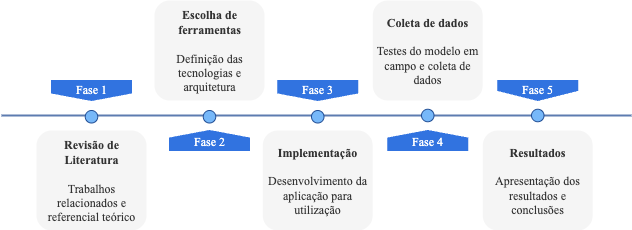
\includegraphics[width=\textwidth]{images/fases_pesquisa.png}
		\fonte{Elaborado pelo autor}
	\end{minipage}
\end{figure}
\FloatBarrier

\section{Modelo Proposto}

Esta seção tem como objetivo descrever brevemente a ferramenta desenvolvida e utilizada para a execução deste trabalho, incluindo sua arquitetura, funcionalidades e tecnologias utilizadas. O modelo proposto consiste em uma aplicação \textit{web} que centraliza as informações do desafio técnico, disponibilizando-o de forma prática e organizada para os desenvolvedores participantes do estudo.

A aplicação coleta o nome e o cargo atual do participante no mercado de trabalho. O nome é utilizado exclusivamente para exibir uma mensagem personalizada de boas-vindas. Funciona como um identificador simples durante a sessão, mantendo o usuário ativo no desafio, sem necessidade de cadastro, \textit{tokens} ou \textit{logins} complexos. Dessa forma, os nomes dos participantes não são utilizados na apresentação dos resultados do estudo, garantindo anonimato e simplicidade na utilização da ferramenta.

\subsection{Visão Geral}

Lorem ipsum.

\subsection{Arquitetura e Tecnologias}

Lorem ipsum.

\subsection{Funcionalidades}

Lorem ipsum.

\subsection{Formulário Inicial}

Lorem ipsum.

\subsection{Tela Inicial e Informações do Desafio}

Lorem ipsum.

\section{Análise e Discussão dos Resultados}

Lorem ipsum.

\subsection{Coleta de Dados}

Lorem ipsum.

\subsection{Avaliação dos Resultados}

Lorem ipsum.

\section{Considerações Finais e Trabalhos Futuros}

Lorem ipsum.

\bibliography{references}

\appendix
\section{DIAGRAMA ER DO BANCO DE DADOS}

Lorem ipsum.

\section{TELAS DA APLICAÇÃO}

Lorem ipsum.

\section{TEXTO TEXTO}

Lorem ipsum.

\section{CENÁRIOS DE TESTES}

Lorem ipsum.

\section{TEXTO TEXTO}

Lorem ipsum.

\section{TEXTO TEXTO}

Lorem ipsum.

\section{RESPOSTAS DO QUESTIONÁRIO}

Lorem ipsum.

\section{REQUISITOS FUNCIONAIS DA APLICAÇÃO}

Lorem ipsum.

\section{TEXTO TEXTO}

Lorem ipsum.

\annex
\section{NOME DO ANEXO}

Lorem ipsum.

\end{document}
